\documentclass{article}
\usepackage[utf8]{inputenc}
\usepackage{amsmath}
\usepackage[spanish]{babel}
\usepackage{graphicx}
\usepackage{float}


\newcommand\tab[1][1cm]{\hspace*{#1}}
\begin{document}



\section*{Problema B}
Nombre: Juan Sebastian Vargas\\
 Codigo: 201215310\\
Fecha: 20/05/16

\section{Algoritmo Soluci\'on}
El Algoritmo consta de una lectura de los datos desde $args\ [i]$ en el método main. Además de esto el algoritmo consta de un metodo para calcula la respuesta, la longitud del periodo, y se basa en obtener los digitos del decimal  multiplicando por 10 el residuo y guardarlo para ver si cuando se repita. Y de esta manera dejar de iterar. 

\section{Complejidades}
En la lectura de datos no tenemos llamadas repetitivas, ya que solo son necesarias para inicializar el programa. \\
Y la complejidad temporal del método que calcula la longitud del periodo es $O(q)$,
Para la complejidad espacial tenemos que guardar todos los residuos, entonces debemos guardar a lo sumo $E(q-1)$ datos.
 

\begin{figure}[h]

 \scalebox{0.65}{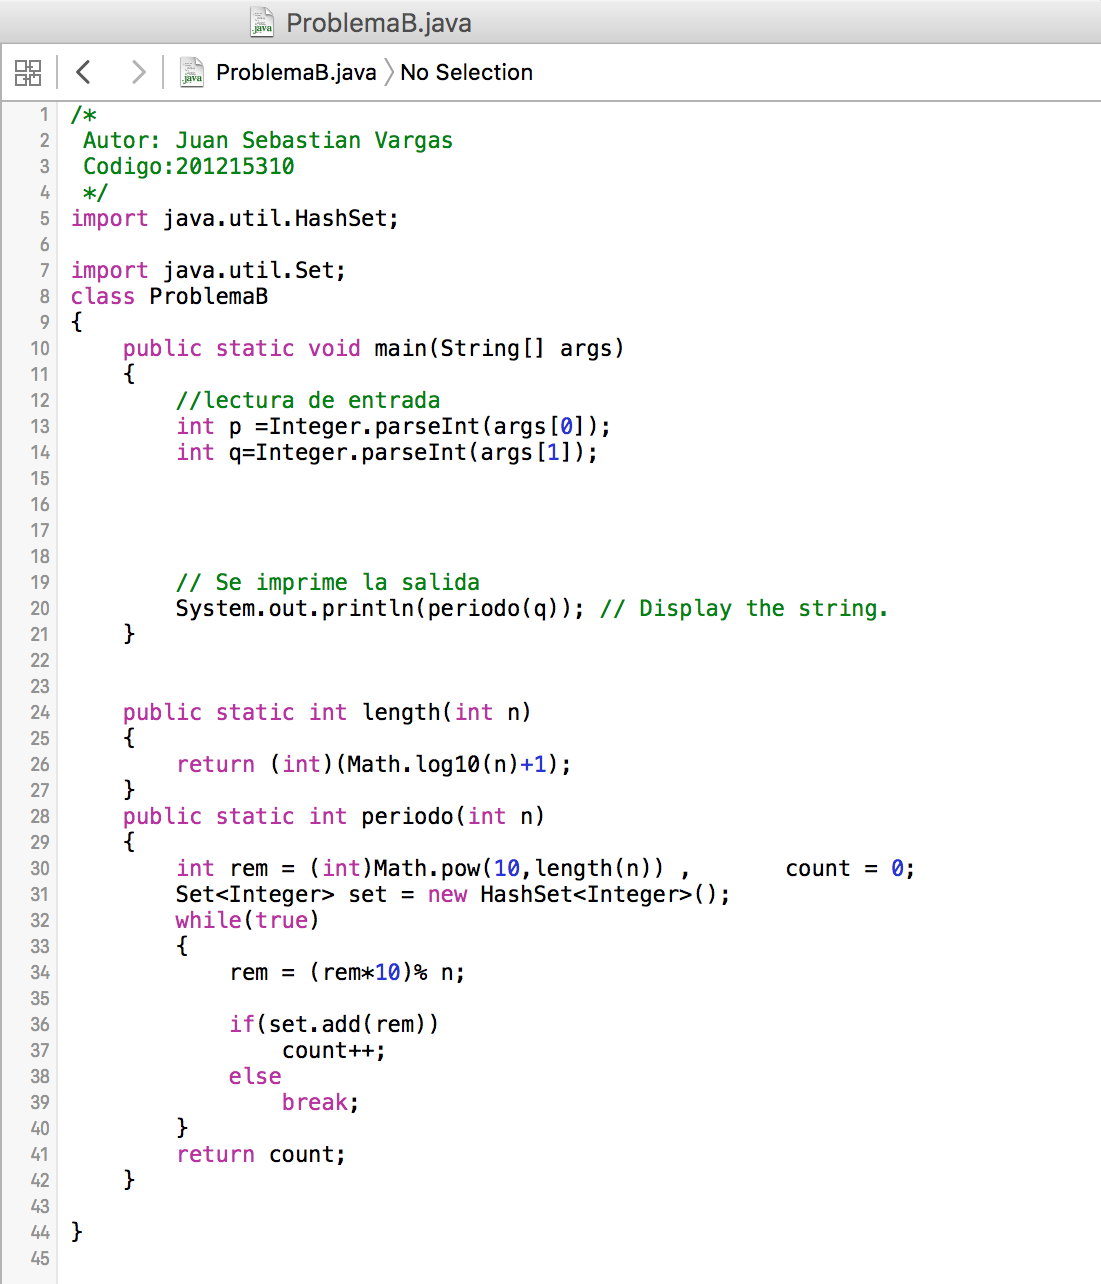
\includegraphics{ProblemaB.png}}
 \label{Al}
 \caption{Algoritmo}
\end{figure}


\end{document}